\documentclass[journal = jacsat,manuscript = note]{achemso}

%% The graphicx package provides the includegraphics command.
%\usepackage{graphicx}
%\usepackage[hidelinks]{hyperref}
%\usepackage{authblk}
\usepackage{natbib}
%\usepackage[backend=bibtex]{biblatex}
\usepackage[T1]{fontenc} % Use modern font encodings
%% The amssymb package provides various useful mathematical symbols
\usepackage{amssymb}

\usepackage{amsmath}

%% The lineno packages adds line numbers. Start line numbering with
%% \begin{linenumbers}, end it with \end{linenumbers}. Or switch it on
%% for the whole article with \linenumbers after \end{frontmatter}.
%\usepackage{lineno}

%\bibliographystyle{plain}
%\addbibresource{plasmid_replication.bib}

\title{How to model DNA replication in stochastic models of synthetic gene circuits (and why)}

\author{Samuel E. Clamons}
\author{Richard M. Murray}
\email{murray@cds.caltech.edu}
\affiliation{Caltech, Pasadena, CA, United States}

%\keywords{Keyword1, Keyword2, Keyword3}

\begin{document}


\begin{abstract}
Biocircuit modeling sometimes requires explicit tracking of a self-replicating DNA species. The most obvious, straightforward way to model a replicating DNA is structurally unstable and leads to pathological model behavior. We describe a simple, stable replication mechanism with good model behavior and show how to derive it from a mechanistic model of ColE1 replication. 
\end{abstract}

\section{Introduction}

Although most synthetic biocircuits use DNA, models of synthetic biocircuits typically do not explicitly describe the dynamics of those DNA species. For example, the original repressilator model tracked mRNA and protein species, but not DNA \cite{elowitz2000}, and the model for the first genetic toggle switch simply tracked ``repressor 1'' and ``repressor 2'' \cite{gardner2000}. For many circuits under many modeling assumptions, it is sufficient to assume that all DNA species are held at a fixed concentration by the cell, by means of mysterious machinery whose details are irrelevant to understanding the circuit.

In some cases, however, it is useful or necessary to explicitly represent DNA as a dynamic species. Some circuits, for example, use DNA in different states as a dynamic component or readout (for example, integrase-based state machines \cite{roquet2016}). Explicit representation of DNA can also be useful when DNA binding is slow relative to the other circuit processes (for example, CRISPR-based transcription factor networks under some conditions \cite{Jones2017}). Stochastic models, in particular, are often most naturally expressed using explicit DNA species.

Explicitly-modeled DNA often requires some mechanism of replication -- again particularly in stochastic models. Unfortunately, the obvious replication implementation $\mathit{DNA} \to \mathit{DNA} + \mathit{DNA}$ is a trap that leads to pathological circuit behavior. 

\section{Trivially-replicating plasmids have no well-defined copy number}

An obvious way to model replication of a DNA species is the straightforward 

$$\mathit{DNA} \overset{\alpha}{\to} \mathit{DNA} + \mathit{DNA}$$

\noindent shown visually in Figure \ref{fig:models_and_traces}A. We refer to this mechanism as ``trivial self-replication''. Although trivial replication is intuitively appealing, we strongly recommend against its use. 

Adding a dilution reaction $\mathit{DNA} \overset{\gamma}{\to} \emptyset$, trivially self-replicating DNA has dynamics

$$\frac{d\mathit{DNA}}{dt} = (\alpha - \gamma) \mathit{DNA}$$

Notice that at steady state, we have $\alpha - \gamma = 0$, \emph{independent of DNA concentration}. In other words, the only finite, non-zero steady state of the trivial replication mechanism occurs when production is precisely balanced by dilution. If production is slightly faster than dilution, then the DNA's concentration will explode unphysically (and unbiologically) to infinity. Conversely, if dilution is slightly faster than production, $\mathit{DNA}$ will always fall to zero concentration and die out. Such a steady state is structurally unstable

In a deterministic model of a trivially-replicating plasmid, production and dilution \emph{can} be balanced perfectly, giving a nominally constant concentration of DNA, but this mechanism of replication rejects no disturbances--any addition or removal of DNA will remain permanently uncorrected.

Stochastic simulations of trivially-replicating DNA cannot even achieve this level of marginal stability. Stochastic simulation is, by its nature, noisy; a stochastically simulated, trivially replicating DNA will random walk in copy number until, practically speaking, it either dies out by wandering to zero or explodes to a concentration too large to simulate (see Figure \ref{fig:models_and_traces}A).

\section{Zero-order replication recovers good steady-state properties}

The trivial replication mechanism is unstable because it has both production and degradation of DNA depend linearly on the concentration of DNA itself. A simple way to add stability to the replication model is to remove that dependence by conditioning replication on a ``dummy replication trigger'' produced at a constant rate (shown diagramatically in Figure \ref{fig:models_and_traces}B):

\begin{align*}
	\emptyset &\overset{\alpha}{\to} R\\
	\mathit{DNA} + R &\overset{k}{\to} \mathit{DNA} + \mathit{DNA}.\\
\end{align*}

\begin{figure}
\centering
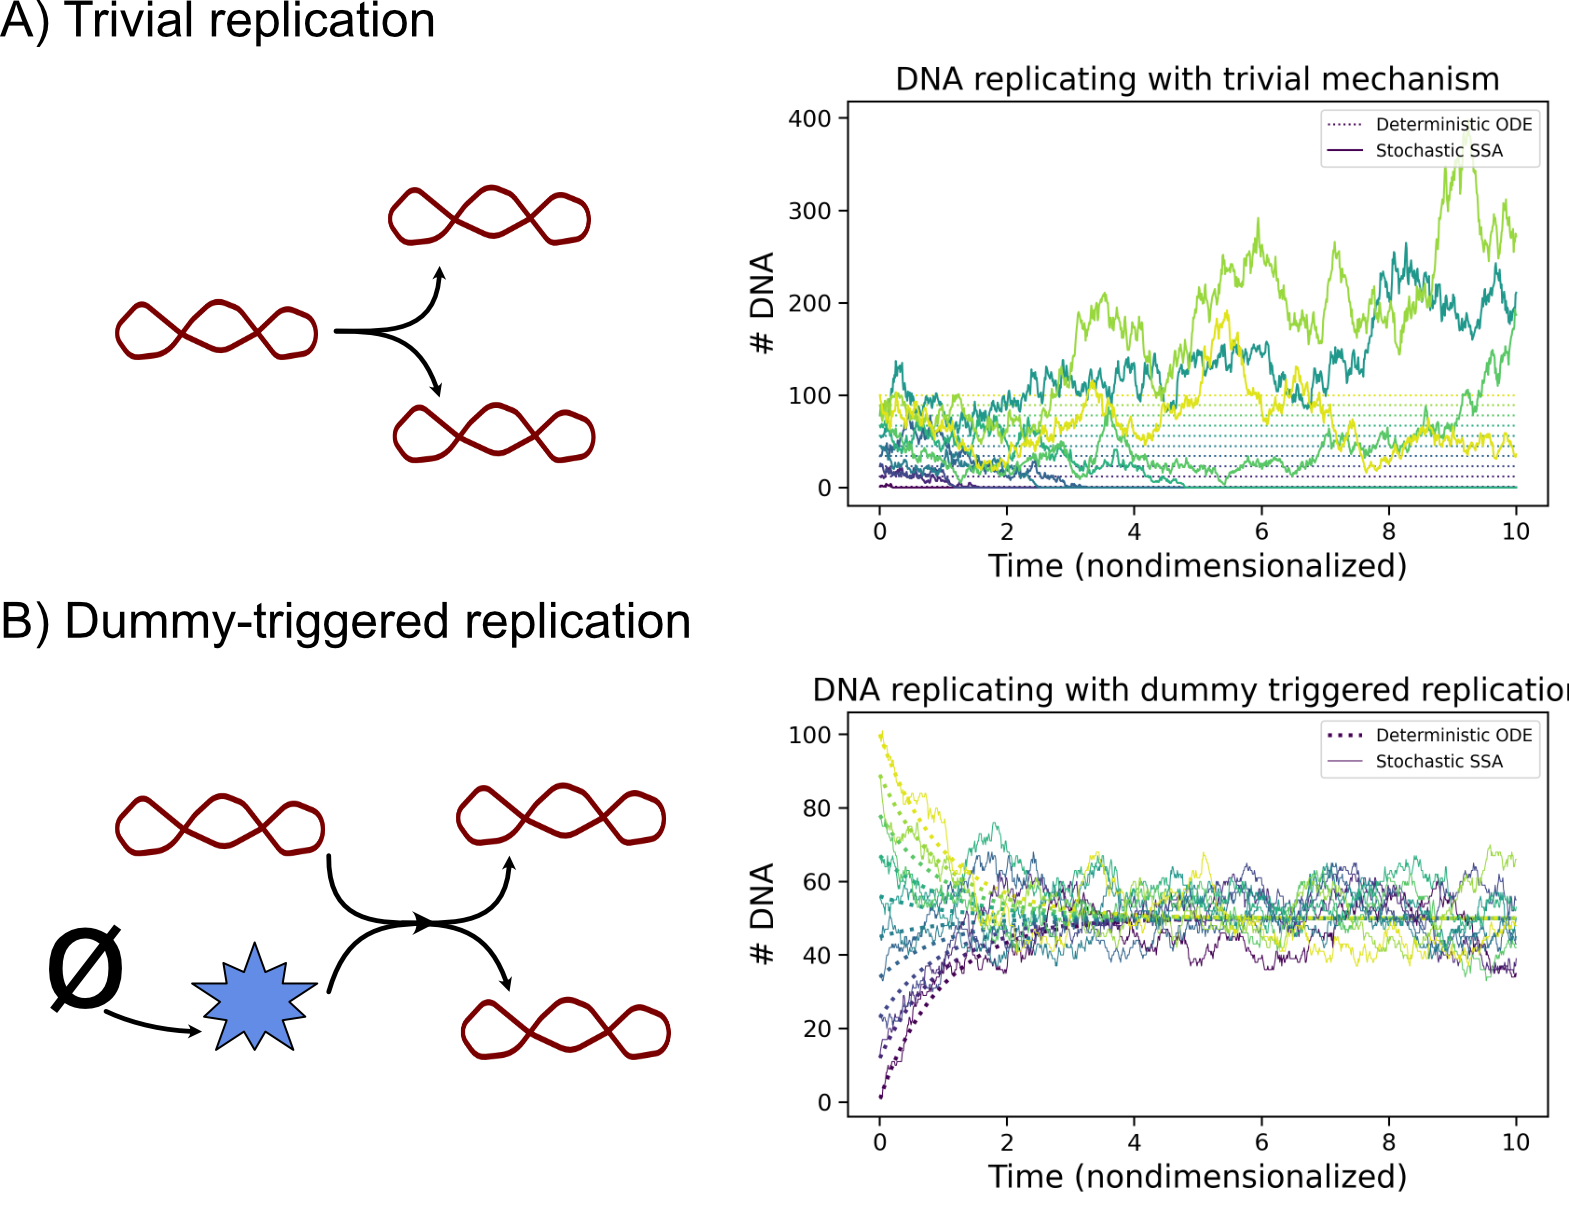
\includegraphics[scale=.75]{figures/models_and_traces.png}
\caption{\textbf{A)} The trivial replication mechanism, in which DNA spontaneously self-replicates. This mechanism is unstable and produces random-walking DNA concentrations. \textbf{B)} The dummy-triggered replication mechanism, in which replication is triggered by a dummy molecule produced at a constant rate. This mechanism, coupled to dilution, is stable and rejects disturbances.}
\label{fig:models_and_traces}
\end{figure}

This mechanism has ODE dynamics

\begin{align*}
\frac{dR}{dt} &= \alpha - kR*\mathit{DNA}\\
\frac{d\mathit{DNA}}{dt} &= kR*\mathit{DNA} - \gamma \mathit{DNA}
\end{align*}

At steady state, $R = \frac{\alpha}{k*\mathit{DNA}}$, which cancels out $\mathit{DNA}$ in $\mathit{DNA}$'s production term and gives $\mathit{DNA} = \frac{\alpha}{\gamma}$. This steady state is stable. As long as $k$ is fast relative to other replication dynamics ($\alpha$ and $\gamma$), the dummy-triggered replication mechanism emulates zero-order replication of DNA.

Because dummy-triggered replication leads to a stable steady state concentration of DNA, as shown in Figure \ref{fig:models_and_traces}B, we recommend it over the trivial replication mechanism.

\section{Biological models of plasmid replication approximately reduce to zero-order replication}\label{sec:reduction}

Dummy-triggered replication is not meant to accurately describe a real biological processes. Real cells do not control replication using consumable molecules like $R$. The critical property of the dummy-triggered replication mechanism is not its realism, but its ability to achieve the (biologically important!) property of having a defined, stable steady state.

Nevertheless, under a few relatively mild assumptions, at least one real-world DNA replication mechanism can be reduced to a zero-order replication mechanism equivalent to the dummy-triggered replication mechanism, . 

Consider the ColE1 plasmid replication system, first crystallized mathematically by Brendel \& Perelson in 1993, shown on the left in Figure \ref{fig:bp_diagram} \cite{Brendel1993}. We use ColE1 as an example because it has a particularly simple and well-understood replication mechanism.

\begin{figure}[h]
\centering
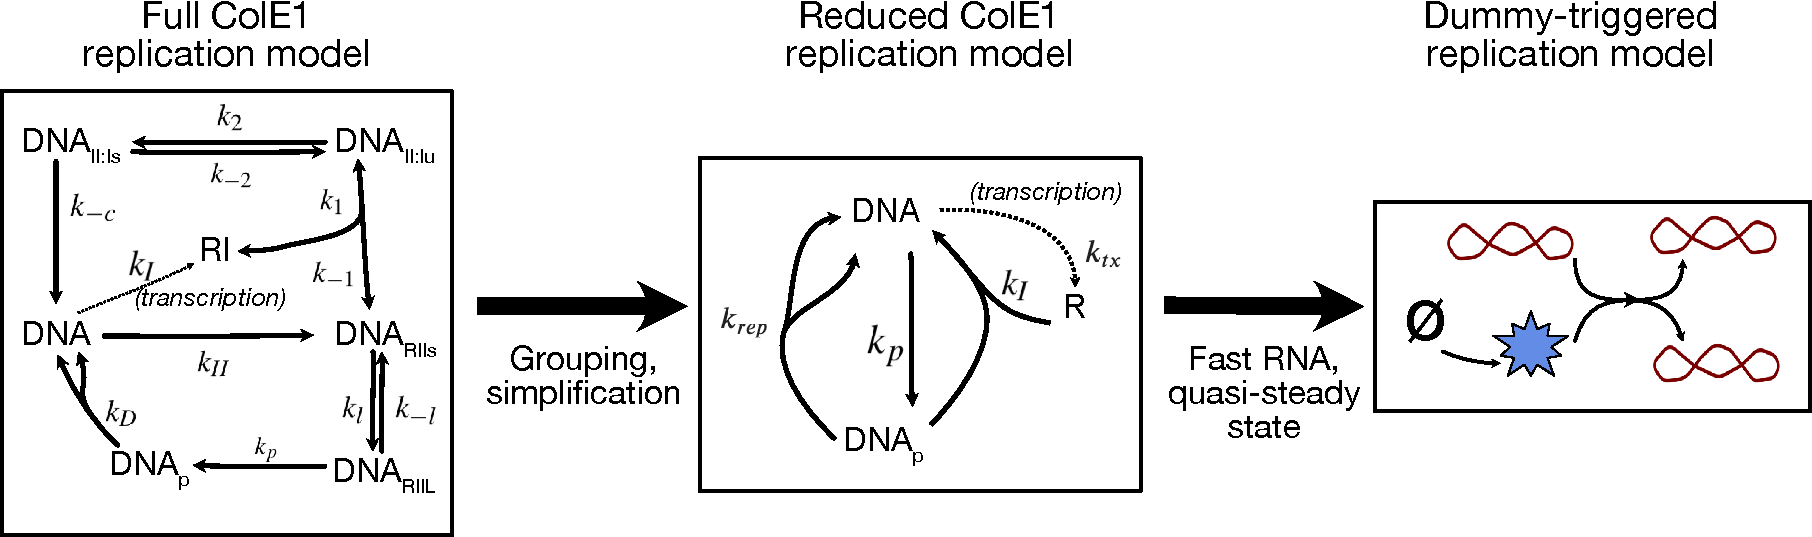
\includegraphics[scale=.4]{figures/bp_diagram.pdf}
\caption{A mechanistic model of ColE1 (left), which can be conceptually approximated by a simplified ColE1 model (middle), which under fast RNA dynamics reduces zero-order replication equivalent to that of the dummy-triggered replication model (right).}
\label{fig:bp_diagram}
\end{figure}

Although the details of the Brendel \& Perelson model are a bit messy, they implement a straightforward logic:

\begin{itemize}
	\item $\mathit{DNA}$ produces an RNA species $RI$. More $\mathit{DNA}$ leads to more $RI$. 
	\item Occasionally, $\mathit{DNA}$ will spontaneously enter a primed state from which it can replicate. (Biologically, the plasmid produces an RNA primer $RNAII$ which can initiate replication.)
	\item $RI$ can react with a replication-primed $\mathit{DNA}$, un-priming it and destroying the $RI$. ($RI$ binds to $RII$ to form an inert complex that is removed by RNases.)
	\item If not stopped by an $RI$, a primed $\mathit{DNA}$ can spontaneously replicate into two non-primed $\mathit{DNA}$. (DNA polymerase initiates replication using $RII$ as a primer.)
\end{itemize}

We can represent this logic more clearly with a three-species reduction of the Brendel \& Perelson model, shown in the middle in Figure \ref{fig:bp_diagram}, consisting of ``unprimed'' $\mathit{DNA}$, ``primed'' $\mathit{DNA}_p$, and feedback RNA $R$. 

We can further simplify the three-species model by assuming that RNA transcription and degradation are fast compared to other replication dynamics. This should be a reasonable assumption, as both $RNAI$ and $RNAII$ have estimated half-lives of $\approx 2$ minutes \cite{Brendel1993}, while the plasmid's doubling time is roughly one \emph{E. coli} cell generation time, or at least $\approx 20$ minutes. Under this assumption, the three-species reduced ColE1 model can be approximated with one of two different single-species models, depending on the relative magnitudes of rate parameters $k_p$ and $k_{rep}$. With $k_{rep}\gg k_p$, total DNA replication rate becomes constant with sufficiently large copy number; when $k_p\gg k_{rep}$, replication rate is always constant. With the right parameterization, we have arrived back at a simple zero-order replication mechanism. 

See supplemental notebook ``simple\_bp\_model\_reduction.ipynb'' for derivations. 

\section{Acknowledgments}

The authors thank John Marken and Andrew Halleran for insightful discussions and thoughtful editing. 

\section{Supporting Information}

For more information and worked examples using the models described here, see our supplementary IPython notebooks at [GITHUB URL]. All notebooks use the BioSCRAPE modeling package to simulate systems with replicating DNA using both standard Gillespie stochastic simulation algorithm (SSA)\cite{Gillespie1977} and a lineage-bjjased simulation algorithm incorporating cell growth and division.

See supplementary notebook ``model\_comparison\_and\_fitting.ipynb'' for:

\begin{itemize}
	\item Full descriptions of the trivial, dummy-triggered replication, full ColE1, and three-species ColE1 models.
	\item Examples of replicating DNA using each of the models with the BioSCRAPE simulation package, 
	\item Replication of Figure \ref{fig:models_and_traces}.
	\item Comparison of model output to empirically-measured plasmid copy numbers taken from \cite{Shao2021}, including parameter inference. 
\end{itemize}

See supplementary notebook ``simple\_bp\_model\_reduction.ipynb'' for:

\begin{itemize}
	\item Derivations of the reductions made in section \ref{sec:reduction}.
	\item Random-parameter simulations evaluating the accuracy of reductions to the three-species reduced ColE1 replication model.
	\item Parameter conditions for stability of the three-species reduced ColE1 model.
\end{itemize}

See supplementary notebook ``CRISPRlator.ipynb'' for:

\begin{itemize}
	\item Worked examples of a 5-node CRISPRi-based repressilator \cite{Clamons2017, Javier2020} implemented on a plasmid using each of the trivial, dummy-triggered replication, full ColE1, and three-species reduced ColE1 models.
	\item Simulations showing synchronization of the CRISPRlator across many generations of growing and dividing cells, and dependence of that synchronization on circuit copy number, using the dummy-triggered replication model.
\end{itemize}

See supplementary notebook ``temporal\_logic\_gate.ipynb'' for:

\begin{itemize}
	\item Worked examples of a population-based DNA integrase circuit capable of sensing the order of and time between arrival of two signals \cite{hsiao2016}.
	\item Demonstration of the same circuit moved to a single cell bearing the circuit on a 30 or 100 copy number plasmid (instead of in many cells bearing a single genomic copy) using dummy-triggered replication.
\end{itemize}

\bibliography{plasmid_replication.bib}

\end{document}
